\subsection{Inflow and outflow for our fictitious cache}
\begin{figure}
\centering
\subfloat[case 1]{
  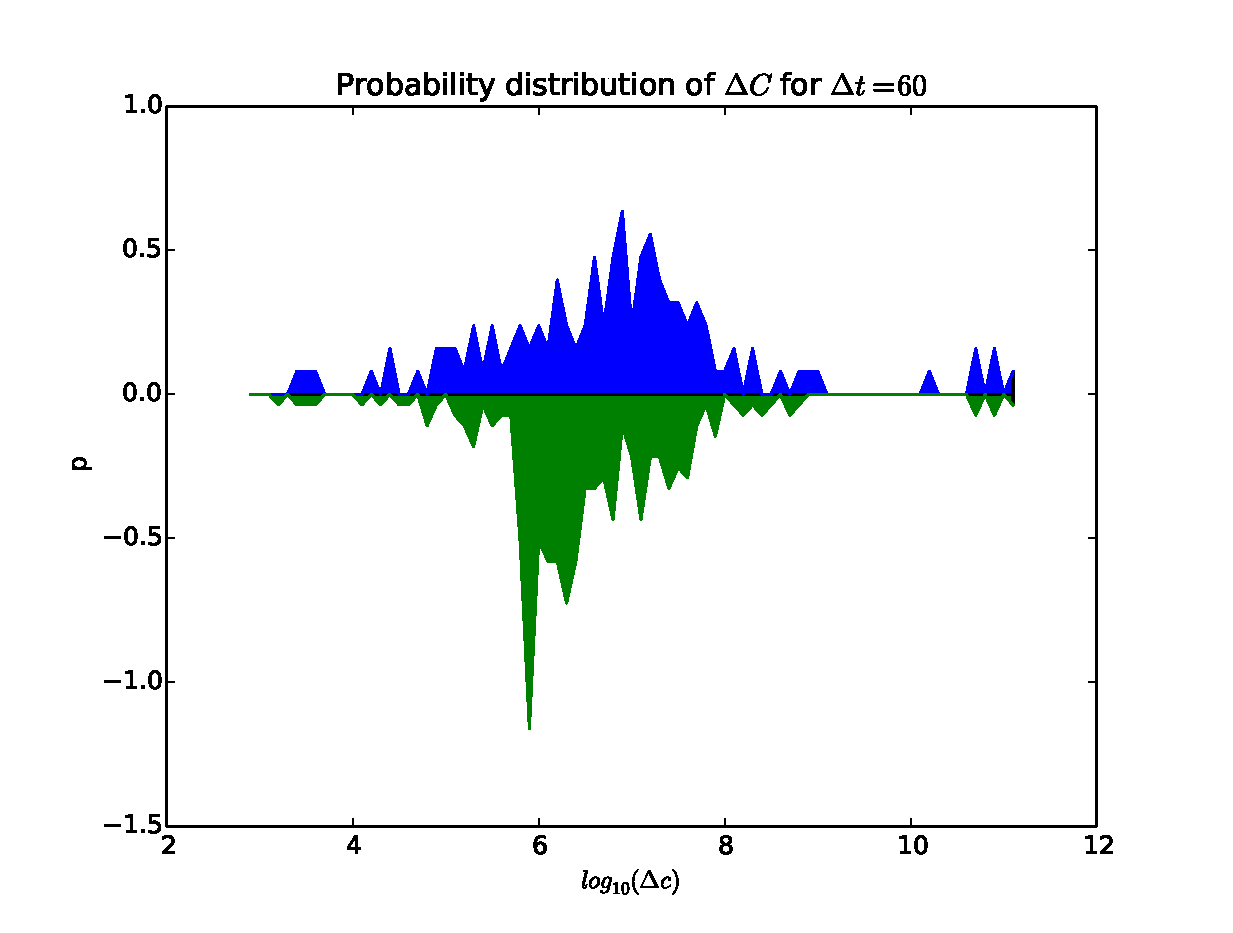
\includegraphics[width=70mm]{ocfa/step4/stripped1_inflow.eps}
}
\subfloat[case 2]{
  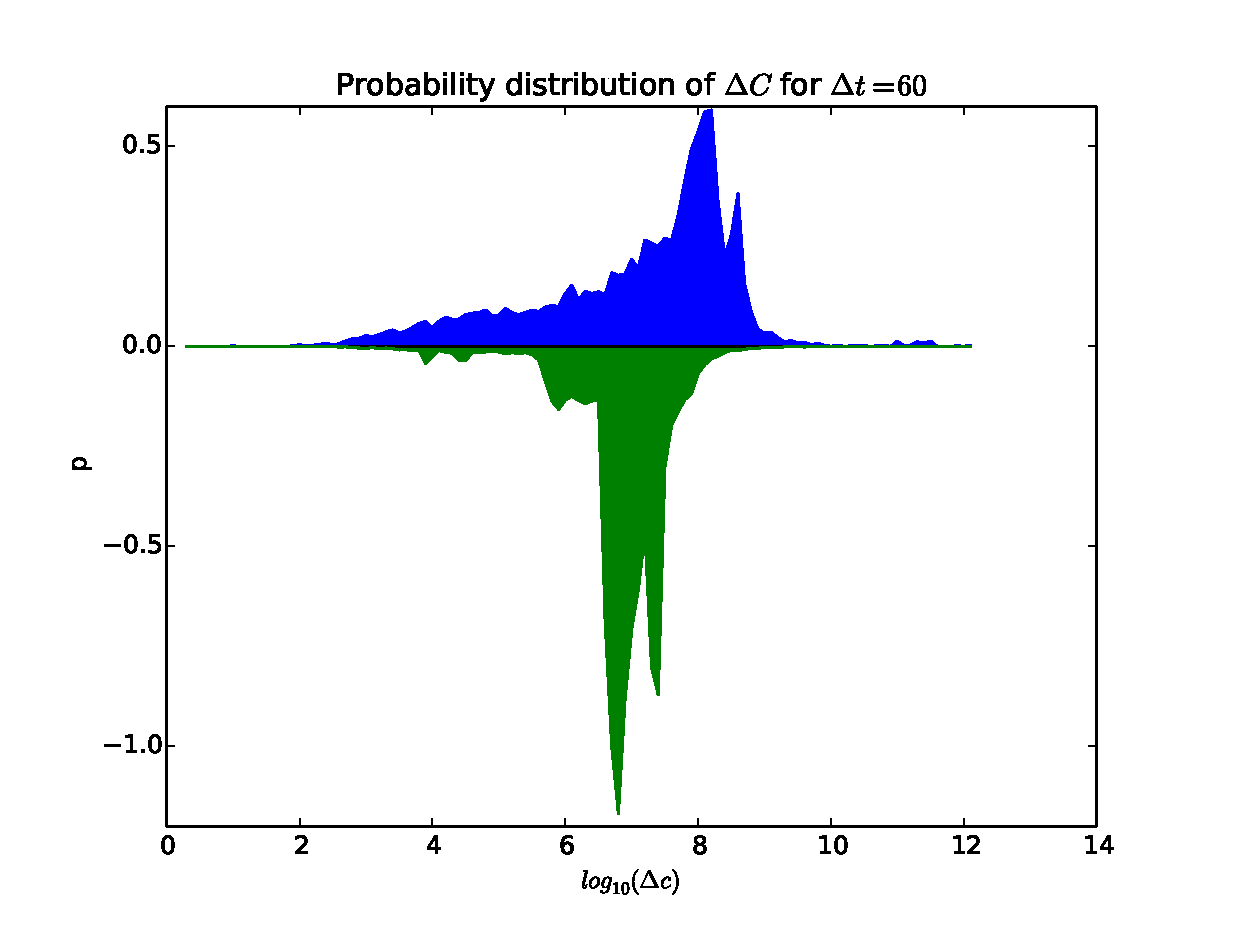
\includegraphics[width=70mm]{ocfa/step4/stripped2_inflow.eps}
}
\hspace{0mm}
\subfloat[case 3]{
  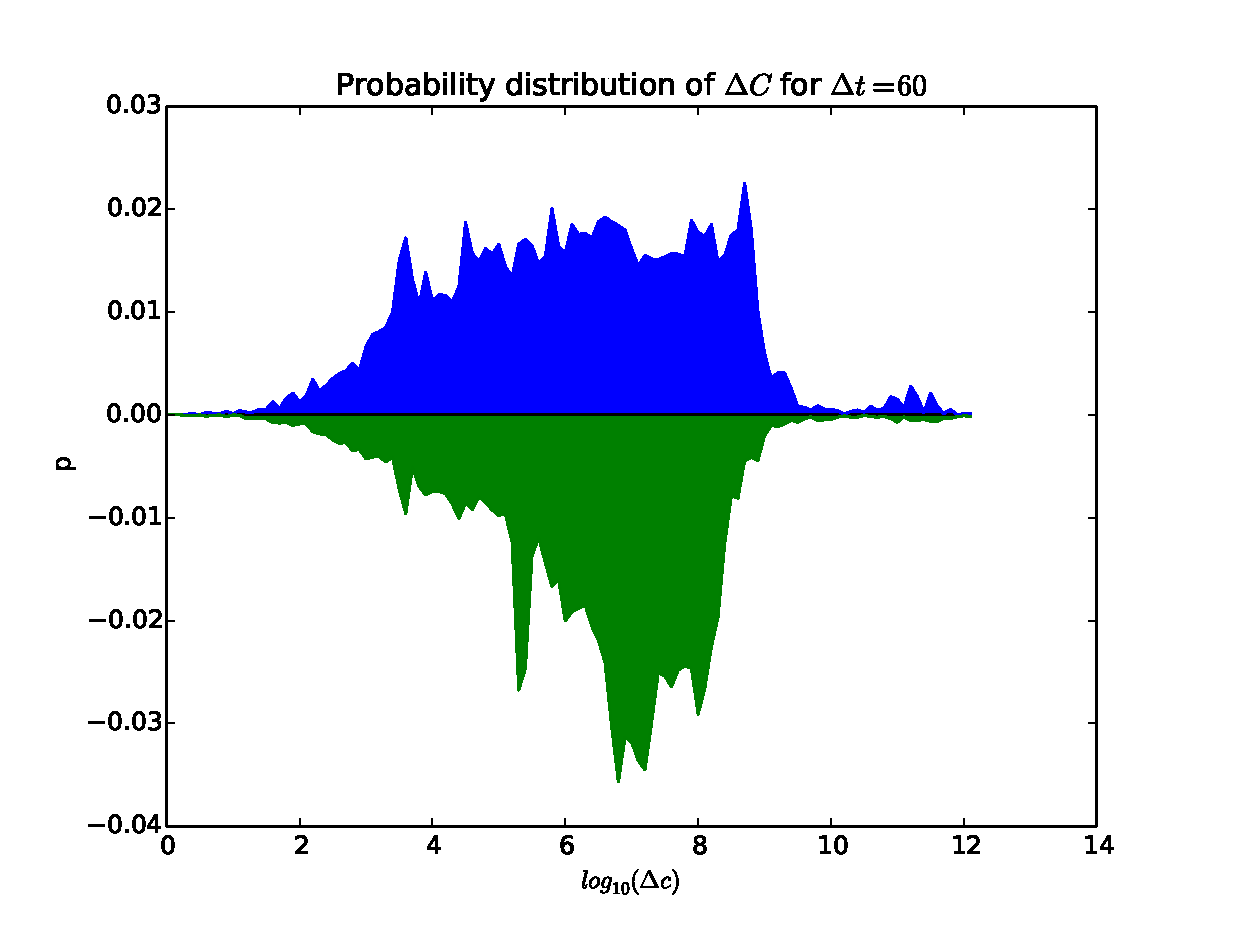
\includegraphics[width=70mm]{ocfa/step4/stripped3_inflow.eps}
}
\subfloat[case 4]{
  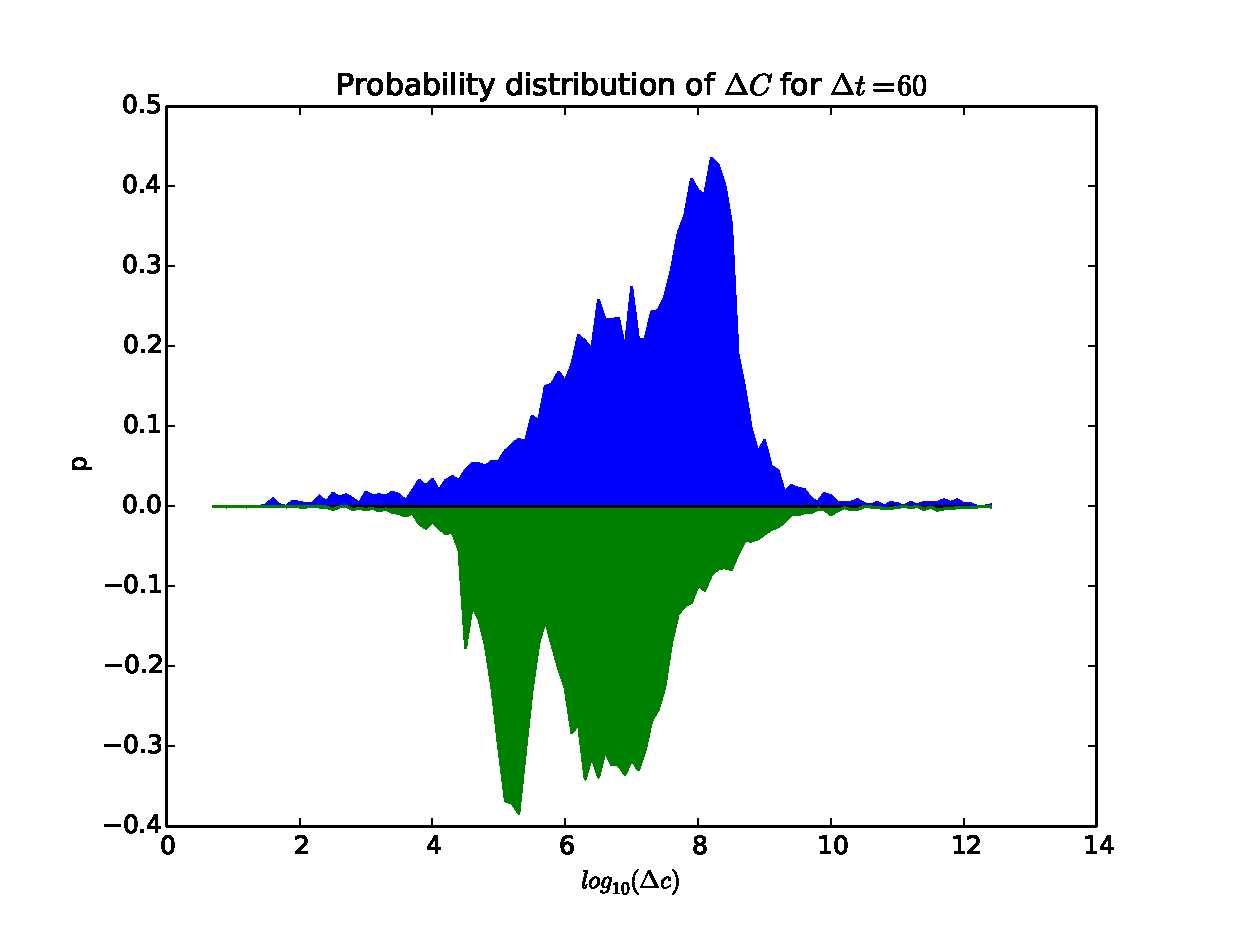
\includegraphics[width=70mm]{ocfa/step4/stripped4_inflow.eps}
}
\caption{In/out flow probability density}
\label{fig:FlowInOut}
\end{figure}
The pictures in ~\ref{fig:FlowInOut} on page ~\pageref{fig:FlowInOut} finally shows the problem with the disk cache misses. It shows both the probability density of growth of the amount of \emph{active} data in the system, and on the negative axis the probability density of shrinkage in one minute intervals. If we remember that this density function is plotted on a logarithmic X, we can identify that the growth density on the upper end of the graphs is higher than the shrinkage density on the upper end of the graph. This means that while there may be many minutes where there is significant shrinkage, the over time amount of \emph{active} data will grow as new data continues being submitted to the system. These results show a clearly that for the OCFA system, there is an imbalance between the data input speed and the overall data processing speed. With knowledge about the investigation, we can further see that the significant production of new evidence data events by modules other than the Java based kickstart, significantly increases the visual noticeable imbalance in these graphs for case two and four.  
